\documentclass[11pt]{book}
\usepackage[T1]{fontenc}
\usepackage[utf8]{inputenc}
\usepackage[english]{babel}
\usepackage{amsmath}
\usepackage{amsfonts}
\usepackage{amssymb}
\usepackage{amsthm}
\usepackage{graphicx}
\usepackage{classicthesis}
\usepackage{arsclassica}

%\let\emph\relax
%\DeclareTextFontCommand{\emph}{\textbf}
\theoremstyle{definition}%per avere lo stile tondo quando uso un ambiente definito da newtheorem
\newtheorem*{defi}{Def}%Definizione per avere la gestione delle definizioni
\newtheorem{prop}{Prop}[chapter]
\newtheorem{thm}{Thm}[chapter]
\newtheorem{esempio}{Esempio}
\newcommand{\numberset}{\mathbb}
\newcommand{\N}{\numberset{N}}
\newcommand{\deriv}{\Rightarrow}
\newcommand{\R}{\numberset{R}}
\newcommand{\transpose}[1]{#1 ^ \mathsf{T}}
\newcommand{\derivative}[1]{\frac{\partial}{\partial #1}}
\newcommand{\myDeriv}[2]{\frac{\partial #1}{\partial #2}}
\newcommand{\gaussian}[2]{\frac{1}{\sqrt{2 \pi #2}} exp \left(\frac{-(y^{(i)} - #1)^2}{2 #2}\right)}

\begin{document}
    \title{Machine Learning Notes}
    \author{Natali Marco}
    \date{}

    \maketitle
    \tableofcontents
    \listoffigures
    
    \chapter{Introduction}


%Chapter 1 Introduction to ML
    \chapter{Linear Regression}
Linear Regression is in statistics a linear process to modeling the relation between
a scalar response (or dependent variable) and one or more explanatory variables (or independent variables).

The case of one explanatory variable is called \emph{simple linear regression} and 
for more than one explanatory variable, the process is called \emph{multiple linear regression}.

Suppose for example we want to predict the price of an house, given living area and the number of bedrooms,
so we represent this relation as a linear regression with the hypothesis function as 
\[ h_{\theta}(x) = \theta_0 + \theta_1 x_1 + \theta_1 x_2 \]
where $x_1$ is the living area and $x_2$ is the number of bedrooms.

Here, the $\theta_i$’s are the parameters(also called \emph{weights}) parameterizing the 
space of linear functions mapping from $x$ to $y$ and when there is no risk of confusion,
we will drop the $\theta$ subscript in $h_{\theta}(x)$ and write it more simply as $h(x)$.

To simplify our notation, we also introduce the convention of letting $x_0 = 1$
(this is the intercept term), so we have 
\[ h_{\theta}(x) = \sum _{i = 0} ^n \theta_i x_i = \transpose{\theta} x \]
where on the right-hand side above we are viewing $\theta$ and $x$ both as vectors, 
and here $n$ is the number of input variables, without counting $x_0$.

\section{Least squares cost function}
Given the training set, to learn $\theta$ parameters a reasonable choice is to make
$h(x)$ close to $y$, at least for the training examples we have.

To formalize this, we will define a function that measures, for each value of the $\theta$’s,
how close the $h(x^{(i)})$’s are to the corresponding $y^{(i)}$’s.

We define the cost function as
\[ J(\theta) = \frac{1}{2} \sum _{i=0} ^n \left (h_{\theta}(x^{(i)}) - y^{(i)} \right )^2 \]
where we divide by $\frac{1}{2}$ in order to simply derivation in future.

If you’ve seen linear regression before, you may recognize this as the familiar 
\emph{least-squares} cost function that gives rise to the ordinary least squares regression model.\newline
Whether or not you have seen it previously, let’s keep going, and we’ll eventually show this to be
a special case of a much broader family of algorithms.

Our objective is to find $\theta$ that minimize $J(\theta)$ so let’s consider now
the \emph{gradient descent} algorithm, which starts with some initial $\theta$, and repeatedly performs the update:
\[ \theta_j = \theta_j - \alpha * \derivative{\theta_j} J(\theta) \]
This update is simultaneously performed for all values of $j= 0, 1, \dots, n$ and 
$\alpha$ is called the \emph{learning rate}.

This is a very natural algorithm that repeatedly takes a step in the direction of steepest decrease of J
and in order to implement this algorithm, we have to work out what is 
the partial derivative term on the right hand side.\newline
Let’s first work it out for the case we have only one training example $(x, y)$, so that we
can neglect the sum in the definition of J and we have 

\begin{align*}
    \derivative{\theta_j} = & \derivative{\theta_j} \frac{1}{2} (h_{\theta}(x) - y)^2 \\
                          = & (h_{\theta}(x) - y) \derivative{\theta_j} (h_{\theta}(x)-y) \\
                          = & (h_{\theta}(x) - y) \derivative{\theta_j} (\sum _{i = 0}^n \theta_i x_i - y) \\
                          = & (h_{\theta}(x) - y)x_j \\
\end{align*}
For a simple training example, it provides the update rule as
\[ \theta_j = \theta_j - \alpha (h_{\theta}(x) - y)x_j ^{(i)} \]
The rule is called the \emph{LMS update rule}(LMS stands for “least mean squares”), and is also known
as the \emph{Widrow-Hoff} learning rule.\newline
This rule has several properties that seem natural and intuitive in fact for instance, the magnitude of 
    the update is proportional to the error term $(y(i) - h_{\theta}(x^{(i)}))$; 
thus, for instance, if we are encountering a training example on which our prediction nearly matches
the actual value of $y^{(i)}$, then we find that there is little need to change the parameters,
in contrast, a larger change to the parameters will be made if our prediction $h_{\theta}(x^{(i)})$ 
has a large error.

We’d derived the LMS rule for when there was only a single training example and 
to modify this method for a training set of more than one example,
we replace the LMS rule with the following algorithm, where we repeat until the convergence the update rule
\[ \theta_j = \theta_j - \alpha (\sum _{i=0}^m (y^{(i)} - h_{\theta}(x^{(i)}) x_j^{(i)} 
   \quad \forall j = 1, 2, \dots, m \]
This is simply gradient descent on the original cost function $J$ and this method looks at every example
in the entire training set on every step, and it is called \emph{batch gradient descent}.\newline
Note that, while gradient descent can be susceptible to local minima in general, the optimization problem
we have posed here for linear regression has only one global, and no other local optima, because 
$J$ is a convex quadratic function.

Another algorithm to train the $\theta$ parameters is \emph{stochastic descent}, where 
we repeatedly run through the training set, and each time we encounter a training example,
we update the parameters according to the gradient of the error with respect to that single training example only.

Whereas batch gradient descent has to scan through the entire training set before taking a single step,
a costly operation if $m$ is large, stochastic gradient descent can start making progress right away,
and continues to make progress with each example it looks at.\newline
Often, stochastic gradient descent gets $\theta$ "close” to the minimum much faster than batch 
gradient descent, but note however that it may never “converge” to the minimum, and the parameters
$\theta$ will keep oscillating around the minimum of $J(\theta)$; in practice most of the values near the minimum
will be reasonably good approximations to the true minimum and for these reasons, particularly when 
the training set is large, stochastic gradient descent is often preferred over batch gradient descent.

\section{Normal Equation}
Gradient Descent gives a way to minimize $J(\theta)$, we present now another method, where 
we performing the minimization explicitly and without resorting to an iterative algorithm.\newline
In this method, we will minimize $J$ by explicitly taking its derivatives with respect to the $\theta_j$’s,
and setting them to zero.\newline
To enable us to do this without having to write pages full of matrices of derivatives,
let’s introduce some notation for doing calculus with matrices.

\subsection{Matrix derivates}
For a function $f: \R ^{m \times n} \to \R$ mapping from $m$-by-$n$ matrices to the real numbers, 
we define the derivative of $f$ with respect to $A$ to be 
\[ \Delta _A f(A) = \begin{bmatrix}
                        \derivative{A_{11}} & \ldots & \derivative{A_{1n}} \\
                        \vdots & \ddots & \vdots \\
                        \derivative{A_{m1}} & \ldots & \derivative{A_{mn}} \\
                    \end{bmatrix} \]
For example suppose $A = \begin{bmatrix}
                       A_{11} & A_{12} \\
                       A_{21} & A_{22} \\
                         \end{bmatrix}$
is a $2 \times 2$ matrix and the function $f:\R ^{2 \times 2} \to \R$ is given by 
\[ f(A) = \frac{3}{2} A_{11} + 5A^2 _{12} + A_{21}A_{22} \]
so we obtain the following gradient matrix 
\[ \Delta _A f(A) = \begin{bmatrix}
                    \frac{3}{2} & 10 A_{12} \\
                    A_{22} & A_{21} \\
                    \end{bmatrix} \]
We also introduce the \emph{trace} operator defined as 
\[ tr A = \sum _{i=1}^n A_{ii} \]
The trace operator has commutative, associative properties and also the following properties(proof is 
easy, you need only to consider the definition) with $A$ and $B$ as square matrices and $a \in \R$
\begin{align*}
    tr A & = tr \transpose{A} \\
    tr (A + B) & = tr A + tr B \\
    tr \, aA & = a \, tr A \\
\end{align*}
We present now some properties about matrix derivation, without proof
\begin{align}
    \Delta _A tr AB & = \transpose{B} \\
    \Delta _{\transpose{A}} f(A) & = \transpose{(\Delta _A f(A))} \\
    \Delta _A tr AB \transpose{A} C & = CAB + \transpose{C} A \transpose{B} \\
    \Delta _A |A| & = |A| \transpose{(A ^{-1})} \\
\end{align}

\subsection{Least squares revised}
Given a training set, define the \emph{design matrix} $X$ to be the $m \times n$ matrix(actually 
the $m \times n+1$ if we include the intercept term), that contains the training example in this way 
\[ X = \begin{bmatrix}
        \dots & \transpose{(x^{(1)})} & \dots \\
        \dots & \transpose{(x^{(2)})} & \dots \\
        \dots & \vdots & \dots \\
        \dots & \transpose{(x^{(m)})} & \dots \\
        \end{bmatrix} \]
Also let $y$ be the $m$ dimensional vector that containing all the target values from the training set
\[ y = \begin{bmatrix}
        y^{(1)} \\
        y^{(2)} \\
        \vdots \\
        y^{(m)} \\
        \end{bmatrix} \]
Now since $h_{\theta}(x) = \transpose{(x^{(i)})} \theta$ we can easily verify that
\[ \begin{bmatrix}
    h_{\theta}(x^{(1)}) - y^{(1)} \\
    \vdots \\
    h_{\theta}(x^{(m)}) - y^{(m)} \\
    \end{bmatrix} \]
Using the fact that for a vector $z$, we have $z ^\intercal z = \sum _i z_i^2$, so we obtain 
\begin{align*}
    \frac{1}{2} \transpose{(X \theta - y)} (X \theta - y) & = \frac{1}{2} \sum _{i = 1}^m
                                                            (h_{\theta}(x^{(i)}) - y^{(i)})^2 \\
                                                        & = J(\theta) \\
\end{align*}
To minimize $J(\theta)$ we consider now the derivative with the respect to $\theta$ 
\begin{align*}
    \Delta _{\theta} J(\theta) & = \Delta _{\theta} \frac{1}{2} \transpose{(X \theta - y)} (X \theta - y) \\
                               & = \frac{1}{2} \Delta _{\theta} (\transpose{\theta} \transpose{X} X \theta -
                                   \transpose{\theta} \transpose{X} y - \theta X \transpose{y} + \transpose{y} y) \\
                               & = \frac{1}{2} \Delta _{\theta} tr(\transpose{\theta} \transpose{X} X \theta -
                                   \transpose{\theta} \transpose{X} y - \theta X \transpose{y} + \transpose{y} y) \\
                               & = \frac{1}{2} \Delta _{\theta} (tr \transpose{\theta} \transpose{X} \theta X -
                                   2 tr \transpose{y} \theta X) \\
                               & = \frac{1}{2} (\transpose{X} X \theta + \transpose{X} X \theta - 2 \transpose{X} y) \\
                               & = \transpose{X} X \theta - \transpose{X} y 
\end{align*}
In the third step, we used the fact that the trace of a real numer is just the real number, the fourth step 
used the fact that $tr A = tr \transpose{A}$ and the fifth step we use the second and third properties given 
in matrix derivation.\newline
To minimize $J$, we set its derivatives to zero, and obtain the normal equations
\[ \transpose{X} X \theta = \transpose{X} y \]
so the value of $\theta$ that minimize $J(\theta)$ is given by 
\[ \theta = (\transpose{X} X)^{-1} \transpose{X} y \]


\section{Probabilistic Interpretation of Linear Regression}
In this section, we will give a set of probabilistic assumptions, under which least-squares regression
is derived as a very natural algorithm and let us assume that the target variables and the inputs 
are related via the equation
\[ y^{(i)} = \transpose{\theta} x + \epsilon ^{(i)} \]
where $\epsilon{(i)}$ is an error term that captures either unmodeled effects, such as if there are some features
very pertinent to predicting housing price, but that we’d left out of the regression, or random noise.

Let us further assume that the $\epsilon^{(i)}$ are distributed IID (independently and identically distributed)
according to a Gaussian distribution as $\epsilon^{(i)} \sim N(0, \sigma^2)$, that implies that 
$P(y^{(i)} | x^{(i)} ; \theta) \sim N(\transpose{\theta}x^{(i)}, \sigma^2)$.

Given $X$, the design matrix, which contains all the $x^{(i)}$’s, and $\theta$, 
the probability of the data is given by $P(y| X; \theta)$ and this quantity is typically viewed 
as a function of $y$, and perhaps $X$, for a fixed value of $\theta$.\newline
When we wish to explicitly view this as a function of $\theta$, we will instead call it the likelihood function
\begin{align*}
    L(\theta) & = L(\theta | X; y) = P(y | X; \theta) \\
              & = \prod _{i = 1} ^ m P(y^{(i)} | x^{(i)}; \theta) \\
              & = \prod _{i = 1} ^ m \gaussian{\transpose{\theta}x^{(i)}}{\sigma ^ 2} \\
\end{align*}

Now, given this probabilistic model relating the $y^{(i)}$’s and the $x^{(i)}$’s, a reasonable way
of choosing our best guess of the parameters $\theta$, we should choose $\theta$ to maximize $L(\theta)$.

Instead of maximizing $L(\theta)$, we can also maximize any strictly increasing function of $L(\theta)$, 
in particular, the derivations will be a bit simpler if we  instead maximize the log likelihood $l(\theta)$
\begin{align*}
    l(\theta) & = \log L(\theta) \\
              & = \log \prod _{i=1} ^ m \gaussian{\transpose{\theta}y^{(i)}}{\sigma ^ 2} \\
              & = \sum _{i = 1} ^ m \log \gaussian{\transpose{\theta}y^{(i)}}{\sigma^2} \\
              & = m \log \frac{1}{\sqrt{2 \pi} \sigma} - 
                  \frac{1}{\sigma^2} \frac{1}{2} \sum _{i=1}^m (y^{(i)} - \transpose{\theta}x^{(i)})^2 \\
\end{align*}
Here maximizing $l(\theta)$ gives the same answer that minimizing
\[ \frac{1}{2} \sum _{i = 1} (y^{(i)} - \transpose{\theta}x^{(i)})^2 \]
which we recognise to be $J(\theta)$, our original least-squares cost function.

Under the previous probabilistic assumptions on the data, least-squares regression corresponds
to finding the maximum likelihood estimate of $\theta$ and this is thus one set of assumptions 
under which least-squares regression can be justified as a very natural method that’s just 
doing maximum likelihood estimation.

Note however that the probabilistic assumptions are by no means necessary for least-squares to be 
a perfectly good and rational procedure, and there may, and indeed there are, other natural assumptions
that can also be used to justify it.

\section{Newton optimization to maximise $l(\theta)$}
Specifically, suppose we have some function $f:\R \to \R$, and we wish to find a value of $\theta$
so that $f(\theta) = 0$.\newline
Here, $\theta \in \R$ is a real number and Newton’s method performs the following update
\[ \theta = \theta - \frac{f(\theta)}{f'(\theta)} \]
This method has a natural interpretation in which we can think of it as approximating the function $f$
via a linear function that is tangent to $f$ at the current guess $\theta$, solving for where that 
linear function equals to zero, and letting the next guess for $\theta$ be where that linear function is zero.

Newton’s method gives a way of getting to $f(\theta) = 0$ and to maximise $l(\theta)$ we have to consider that
the maxima of $l$ correspond to points where its first derivative $l'(\theta)$ is zero.\newline
So, by letting $f(\theta) = l'(\theta)$, we can use the same algorithm to maximize $l$, and we obtain the update rule
\[ \theta = \theta - \frac{l'(\theta)}{l''(\theta)} \]
The generalization of Newton’s method to multidimensional setting(also called the \emph{Newton-Raphson} method)
is given by 
\[ \theta = \theta - H^{-1} \Delta _{\theta} \, l(\theta) \]
where $H^{-1}$ is the second derivative called \emph{Hessian}.

Newton’s method typically enjoys faster convergence than (batch) gradient descent, and requires
many fewer iterations to get very close to the minimum.\newline
One iteration of Newton’s can, however, be more expensive than one iteration of gradient descent,
since it requires finding and inverting an $n \times n$ Hessian; but so long as $n$ is not too large,
it is usually much faster over all.\newline
When Newton’s method is applied to maximize the logistic regression log likelihood function $l(\theta)$,
the resulting method is also called \emph{Fisher scoring}.

\section{Locally Weighted Regression}
Learning algorithms can be divided in two different categories:
\begin{description}
    \item [Parametrics:] fit fixed set of parameters $\theta$ to data
    \item [Non parametrics:] you have to keep an amount of data/parameters, that grows with size of data
\end{description}
\emph{Locally Weight Regression} is our first example of non parametric learning algorithm, where to predict
from a point $x_i$ you have to watch their neighbors.

The objective is to fit $\theta$ to minimize the objective function
\[ \sum _{i = 1}^n w^{(i)}(y^{(i)} - \transpose{\theta}x^{(i)})^2 \]
where $w^{(i)}$ is a weight function and a common choice of weight function is the following
\[ w^{(i)} = exp \left(\frac{-(x^{(i)} - \hat{x})^2}{2 \tau ^ 2}\right) \]
Note that the weights depend on the particular point $x$ at which we’re trying to evaluate $x$ so
if $|x^{(i)} - \hat{x}|$ is small the weight is close to 1, instead if $|x^{(i)} - \hat{x}|$ is 
large the weight is close to $0$.

Hence, $\theta$ is chosen giving a much higher “weight” to the (errors on) training examples close
to the query point $x$ and note also that while the formula for the weights takes a form that is 
cosmetically similar to the density of a Gaussian distribution, the $w(i)$’s do not directly have anything
to do with Gaussians, and in particular the $w(i)$ are not random variables, normally distributed or otherwise.

The parameter $\tau$ controls how quickly the weight of a training example falls off with distance of
its $x^{(i)}$ from the query point $x$ and it is called the \emph{bandwidth} parameter, which choice of value
is important to avoid overfitting and underfitting.

It is commonly used when we have a lot of data and we don't want to think about which features to use.


%Chapter 2 Linear Regression
    \chapter{Classification}
In statistics \emph{Classification} is the problem of identifying to which of a set of categories(sub-populations)
a new observation belongs, on the basis of a training set of data containing observations 
whose category membership is known.

Examples are assigning a given email to the "spam" or "non-spam" class, assigning a diagnosis
to a given patient based on observed characteristics of the patient(sex, blood pressure, presence 
or absence of certain symptoms, etc.) and classification is an example of pattern recognition.

In the terminology of machine learning, classification is considered an instance of supervised learning, 
in which we learn based on training set of correctly identified observations.

For now, we will focus on the binary classification problem in which $y$ can take on only two values,
$0$ and $1$, but most of what we say here will also generalize to the multiple-class case.\newline
For instance, if we are trying to build a spam classifier for email, then $x^{(i)}$ may be some features
of a piece of email, and $y$ may be $1$ if it is a piece of spam mail, and $0$ otherwise.\newline
$0$ is also called the \emph{negative class}, and $1$ the \emph{positive class} and
given $x^{(i)}$, the corresponding $y^{(i)}$ is also called the \emph{label} for the training example.

\section{Logistic Regression}
We could approach the classification problem ignoring the fact that $y$ is discrete-valued,
and use our old linear regression algorithm to try to predict $y$ given $x$.\newline
However, it is easy to construct examples where this method performs very poorly, in fact intuitively,
it also doesn’t make sense for $h_{\theta}(x)$ to take values larger than $1$ or smaller than $0$
when we know that $y \in \{0,1\}$.

To fix this, let’s change the form for our hypotheses $h_{\theta}(x)$ and we will choose
\[ h_{\theta}(x) = g(\transpose{\theta} x) = \frac{1}{1 + e^{-\transpose{\theta} x}} \]
where is called \emph{sigmoid function} the equation
\[ g(z) = \frac{1}{1 + e^{-z}} \]

In figure \ref{img:sigmoid} is showed the function $g(z)$, where $g(z)$ tends to $1$ as $z \to \infty$ 
and tends to $0$ as $z \to -\infty$.

\begin{figure}
    \caption{Representation of Sigmoid function}
    \label{img:sigmoid}
    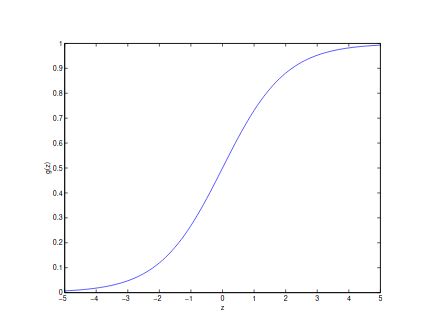
\includegraphics{images/sigmoid}
\end{figure}
For now, let’s take the choice of $g$ as given, in fact other functions that smoothly increase from $0$ to $1$
can also be used, but for a couple of reasons that we’ll see later, when we talk about GLMs, 
and when we talk about generative learning algorithms, the choice of the logistic function is a fairly natural one.

Before moving on, here’s a useful property of the derivative of the sigmoid function, which we write as $g'$
\begin{align*}
    g' & = \derivative{z} \frac{1}{1 + g^{-z}} \\
       & = \frac{1}{(1 + e^{-z})^2} (e^{-z}) \\
       & = \frac{1}{1 + e^{-z}} (1 - \frac{1}{1 + e^{-z}}) \\
       & = g(z) (1 - g(z)) 
\end{align*}
So, given the logistic regression model, to fit $\theta$ we follow how we saw least squares regression 
could be derived as the maximum likelihood estimator under a set of assumptions, let’s endow our 
classification model with a set of probabilistic assumptions, and then fit the parameters via maximum likelihood.

Let us assume that 
\begin{align*}
    P(y = 1 | x; \theta) & = h_{\theta}(x) \\
    P(y = 0 | x; \theta) & = 1 - h_{\theta}(x) \\
\end{align*}
Assuming that the $m$ training examples were generated independently, we can then write down the 
likelihood of the parameters as
\begin{align*}
    L(\theta) & = p(y | x; \theta) \\
              & = \prod _{i = 1}^m p(y^{(i)} | x^{(i)}; \theta) \\
              & = \prod _{i = 1}^m (h_{\theta}(x^{(i)}))^{y^{(i)}} (1 - h_{\theta}(x^{(i)}))^{1 - y^{(i)}} \\
\end{align*}
As before, it is more easy to maximise the log lihelikood 
\begin{align*}
    l(\theta) & = \log L(\theta) \\
              & = \prod _{i=1}^m y^{(i)} \log h_{\theta}(x^{(i)}) + (1 - y^{(i)}) \log (1 - h_{\theta}(x^{(i)})) \\
\end{align*}
Similar to our derivation in the case of linear regression, we can use \emph{gradient ascent} and 
written invectorial notation, our updates will therefore be given by
\[ \theta = \theta + \alpha \, \Delta _{\theta} \, l(\theta) \]
Let’s start by working with just one training example $(x, y)$, and take derivatives to derive
the stochastic gradient ascent rule
\begin{align*}
    \derivative{\theta_j} l(\theta) & = \left(y \frac{1}{g(\transpose{\theta} x)} - 
                                        (1 - y) \frac{1}{1 - g(\transpose{\theta} x)}\right) 
                                        \derivative{\theta_j} g(\transpose{\theta} x) \\
                                    & = \left(y \frac{1}{g(\transpose{\theta} x)} - 
                                        (1 - y) \frac{1}{1 - g(\transpose{\theta} x)}\right)
                                        g(\transpose{\theta} x)(1 - g(\transpose{\theta} x)
                                        \derivative{\theta_j} \transpose{\theta} x \\
                                    & = (y (1 - g(\transpose{\theta} x)) - (1-y) g(\transpose{\theta} x)) x_j \\
                                                 & = (y - h_{\theta}(x))x_j \\
\end{align*}
Above we used the fact that $g'(x) = g(x)(1-g(x))$ and therefore it gives us the stochastic gradient ascent rule
\[ \theta_j = \theta_j + \alpha (y - h_{\theta}(x))x_j \]
If we compare this to the LMS update rule, we see that it looks identical, but this is not 
the same algorithm, because $h_{\theta}(x^{(i)})$ is now defined as a non-linear function.\newline
Nonetheless, it’s a little surprising that we end up with the same update rule for a rather different algorithm
and learning problem, as how we will deeper talk in GLM(Generalized Linear Models) chapter.

\section{Perceptron algorithm}
We now digress to talk briefly about an algorithm that’s of some historical interest, 
and that we will also return to later when we talk about learning theory.\newline
Consider modifying the logistic regression method to “force” it to output values that are either $0$ or $1$.

To do so, it seems natural to change the definition of $g$ to be the threshold function

\[ g(z) = \begin{cases}
            1 \quad x \geq 0 \\
            0 \quad x < 0 \\
          \end{cases} \]

In the 1960s, this “perceptron” was argued to be a rough model for how individual neurons in the brain work and 
given how simple the algorithm is, it will also provide a starting point for our analysis when we talk
about learning theory later.

Note however that even though the perceptron maybe cosmetically similar to the other algorithms we talked about,
it is actually a very different type of algorithm than logistic regression and least squares linear regression;
in particular, it is difficult to endow the perceptron’s predictions with meaningful probabilistic interpretations,
or derive the perceptron as a maximum likelihood estimation algorithm.

%Chapter 3 Classification
    \chapter{Generalized Linear Models}
So far, we’ve seen a regression example, and a classification example: in the regression example, we had
$y | x; \theta \sim N(\mu, \sigma^2)$, and in the classification one $y | x; \theta \sim Bernoulli(\phi)$,
for some appropriate definitions of $\mu$ and $\phi$ as functions of $x$ and $\theta$.

In this section, we will show that both of these methods are special cases of a broader family of models,
called \emph{Generalized Linear Models}(GLMs) and we will also show how other models in the GLM family
can be derived and applied to other classification and regression problems.

\section{Exponential family}
To work our way up to GLMs, we will begin by defining exponential family distributions and we say that
a class of distributions is in the exponential family if it can be written in the form
\[ P(y | \eta) = b(y) \, exp(\eta^T T(y) - a(\eta)) \]
Here, $\eta$ is called the \emph{natural parameter} of the distribution, $T(y)$ is the 
sufficient statistic(for the distributions we consider, it will often be the case that $T(y) = y$),
$a(\eta)$ is the \emph{log partition} function and the quantity $e^{a(\eta)}$ essentially plays the role
of a normalization constant, that makes sure the distribution $p(y | \eta)$ sums/integrates over $y$ to 1.

A fixed choice of $T,a$ and $b$ defines a family(or set) of distributions that is parameterized by $\eta$;
as we vary $\eta$, we then get different distributions within this family and we now show that the Bernoulli
and the Gaussian distributions are examples of exponential family distributions.

The Bernoulli distribution with mean $\phi$, written $Bernoulli(\phi)$, specifies a distribution 
over $y \in \{0,1\}$, so that $p(y = 1 | \phi) = \phi$ and $p(y = 0 | \phi) = 1 - \phi$.\newline
As we vary $\phi$, we obtain Bernoulli distributions with different means and we now show that this class
of Bernoulli distributions, ones obtained by varying $\phi$, is in the exponential family.

We write the Bernoulli distribution as
\begin{align*}
    P(y | \phi) & = \phi ^ y (1 - \phi)^{1 - y} \\
                & = exp(\log(\phi^y (1 - \phi)^{1 - y})) \\
                & = exp \left(\log \left(\frac{\phi}{1-\phi}\right)y + \log (1 - y)\right) \\
\end{align*}
Thus, the natural parameter is given by $\eta= \log(\frac{\phi}{1-\phi})$ and it is interestingly,
if we invert this definition for $\eta$ by solving for $\phi$ in terms of $\eta$, we obtain
\[ \phi = \frac{1}{1 + e ^ {-\eta}} \]
This is the familiar sigmoid function and this will come up again when we derive logistic regression as a GLM.

To complete the formulation of the Bernoulli distribution as an exponential family distribution, we also have
\begin{align*}
    T(y) & = y \\
    a(\eta) & = - \log (1 - \phi) \\
            & = \log (1 + e^{\eta}) \\
    b(y) & =  1 \\
\end{align*}
Let’s now move on to consider the Gaussian distribution and recall that, when deriving linear regression, 
the value of $\sigma ^ 2$ had no effect on our final choice of $\theta$ and $h_{\theta}(x)$.

Thus, we can choose an arbitrary value for $\sigma^2$ without changing anything and to simplify the derivation below,
let’s set $\sigma^2 = 1$, so we have
\begin{align*}
    P(y | \mu) & = \frac{1}{\sqrt{2 \pi}} exp \left(-\frac{1}{2} (y - \mu)^2 \right) \\
               & = \frac{1}{\sqrt{2 \pi}} exp \left(-\frac{y^2}{2}\right) exp\left(\mu y - \frac{\mu^2}{2}\right) \\
\end{align*}
Thus, we see that the Gaussian is in the exponential family, with
\begin{align*}
    \eta & = \mu \\
    T(y) & = y \\
    b(y) & = \frac{1}{\sqrt{2 \pi}} exp(\frac{-y^2}{2}) \\
    a(\eta) & = \frac{\mu^2}{2} = \frac{\eta^2}{2} \\
\end{align*}
There’re many other distributions that are members of the exponential family: 
the multinomial, the Poisson (for modelling count data),
the gamma and the exponential (for modelling continuous, non-negative random variables, such as time-intervals),
the beta and the Dirichlet (for distributions over probabilities) and many more.\newline
In the next section, we will describe a general “recipe” for constructing models in which $y$ 
(given $x$ and $\theta$) comes from any of these distributions.

\section{Constructing GLM}
Suppose you would like to build a model to estimate the number $y$ of customers arriving in your store
(or number of page views on your website) in any given hour, based on certain features $x$ 
such as store promotions, recent advertising, weather, day of week, etc.

We know that the Poisson distribution usually gives a good model for numbers of visitors and knowing this,
how can we come up with a model for our problem? Fortunately, the Poisson is an exponential family distribution,
so we can apply a Generalized Linear Model(GLM).\newline
In this section, we will describe a method for constructing GLM models for problems such as these and 
more generally, consider a classification or regression problem where we would like to predict the value 
of some random variable $y$ as a function of $x$.

To derive a GLM for this problem, we will make the following three assumptions about the conditional distribution
of $y$ given $x$ and about our model:
\begin{enumerate}
    \item $y;x, \theta \sim ExponentialFamily(\eta)$.
    \item Given $x$, our goal is to predict the expected value of $T(y)$ given $x$ and 
          in most of our examples, we will have $T(y) = y$, so this means we would like the prediction $h(x)$
          output by our learned hypothesis $h$ to satisfy $h(x) = E[y | x]$.
    \item The natural parameter $\eta$ and the inputs $x$ are related linearly $\eta = \transpose{\theta}x$;
          if $\eta$ is vector valued, then $\eta_i = \transpose{\theta_i}x$.
\end{enumerate}
The third of these assumptions might seem the least well justified of the above, and it might be better thought
of as a “design choice” in our recipe for designing GLMs, rather than as an assumption per se and 
these three assumptions/design choices will allow us to derive a very elegant class of learning algorithms,
namely GLMs, that have many desirable properties such as ease of learning.

Furthermore, the resulting models are often very effective for modelling different types of distributions over $y$;
for example, we will shortly show that both logistic regression and ordinary least squares can both be derived as GLMs.

\subsection{Ordinary Least Squares}
To show that ordinary least squares is a special case of the GLM family of models, consider the setting 
where the target variable $y$ (also called the \emph{response variable} in GLM terminology) is continuous,
and we model the conditional distribution of $y$ given $x$ as a Gaussian $N(\mu, \sigma^2)$.

So, we let the ExponentialFamily($\eta$) distribution above be the Gaussian distribution and 
as we saw previously, in the formulation of the Gaussian as an exponential family distribution,
we had $\mu = \eta$ and so we have
\begin{align*}
    h_{\theta}(x) & = E[y | x; \theta] \\
                  & = \mu \\
                  & = \eta \\
                  & = \transpose{\theta} x \\
\end{align*}

\subsection{Logistic Regression}
We now consider logistic regression and here we are interested in binary classification, so $y \in \{0,1\}$.

Given that $y$ is binary valued, it therefore seems natural to choose the Bernoulli family of distributions
to model the conditional distribution of $y$ given $x$ and in our formulation of the Bernoulli distribution as
an exponential family distribution, we had $\phi = \frac{1}{1 + e ^{-\eta}}$.

Furthermore, note that if $y | x; \theta \sim Bernoulli(\phi)$, then $E[y | x; \theta] = \phi$, so following
a similar derivation as the one for ordinary least squares, we get
\begin{align*}
    h_{\theta}(x) & = E[y | x; \theta] \\
                  & = \phi \\
                  & = \frac{1}{1 + e ^ {-\eta}} \\
                  & = \frac{1}{1 + e ^ {-\transpose{\theta} x}} \\
\end{align*}
So, this gives us hypothesis functions of the form 
\[ h_{\theta}(x) = \frac{1}{1 + e^{-\transpose{\theta} x}} \].

To introduce a little more terminology, the function $g$ giving the distribution’s mean as a function 
of the natural parameter ($g(\eta) = E[T(y); \eta]$) is called the \emph{canonical response function}.\newline
Its inverse, $g^{-1}$, is called the \emph{canonical link function} and thus, the canonical response function
for the Gaussian family is just the identify function and the canonical response function for the Bernoulli
is the logistic function.

\section{Softmax Regression}
Consider a classification problem in which the response variable $y$ can take on any one of $k$ values,
so $y \in \{1, 2, \dots, k\}$; for example, rather than classifying email into the two classes 
spam or not spam, which would have been a binary classification problem, we might want to classify it
into three classes, such as spam, personal mail, and work related mail.\newline
The response variable is still discrete, but can now take on more than two values and we will thus model it 
as distributed according to a multinomial distribution.

Let’s derive a GLM for modelling this type of multinomial data and to do so, we will begin by expressing
the multinomial as an exponential family distribution.\newline
To parameterize a multinomial over $k$ possible outcomes, one could use $k$ parameters $\phi_1, \dots, \phi_k$ 
specifying the probability of each of the outcomes, however, these parameters would be redundant, or more formally,
they would not be independent, since knowing any $k-1$ of the $\phi_i$’s uniquely determines the last one,
as they must satisfy $\displaystyle \sum _{i = 1}^k \phi_i = 1$.

So, we will instead parameterize the multinomial with only $k-1$ parameters $\phi_1, \dots, \phi_{k-1}$, 
where $\displaystyle \phi_i =P(y=i; \phi)$, and $\displaystyle P(y = k; \phi) = 1 - \sum _{i=1}^{k-1} \phi_i$.\newline
For notational convenience, we will also let $\displaystyle \phi_k= 1 - \sum _{i=1}^{k-1} \phi_i$, 
but we should keep in mind that this is not a parameter, and that it is fully specified by $k-1$ parameters.\newline
To express the multinomial as an exponential family distribution, we will define $T(y) \in \R ^{k-1}$ in which 
$T_i$ has $0$ in all entries except $1$ in $i$-th row.

Unlike our previous examples, here we do not have $T(y) = y$ and also, $T(y)$ is now a $k-1$ dimensional vector,
rather than a real number.\newline
We will write $(T(y))_i$ to denote the $i$-th element of the vector $T(y)$.\newline
We introduce one more very useful piece of notation: an indicator function $1\{*\}$ takes on a value of $1$
if its argument is true, and $0$ otherwise ($1\{True\} = 1, 1\{False\} = 0$).

So, we can also write the relationship between $T(y)$ and $y$ as $(T(y))_i = 1\{y=i\}$ and 
further, we have that $E[(T(y))_i] = P(y=i) = \phi_i$.\newline
We are now ready to show that the multinomial is a member of the exponential family, infact we have
\begin{align*}
    P(y | \phi) & = \phi _1^{1\{y=1\}} \phi_2^{1\{y=2\}} \dots \phi_k^{1\{y=k\}} \\
               & = \phi _1^{1\{y=1\}} \phi_2^{1\{y=2\}} \dots \phi_k^{1 - \sum _{i=1}^{k-1} 1\{y = i\}} \\
               & = \phi_1^{(T(y))_1} \phi_2^{(T(y))_2} \dots \phi_k^{1 - \sum _{i=1}^{k-1} (T(y))_i} \\
               & = exp \left((T(y))_1 \log \phi_1 + (T(y))_2 \log \phi_2 + \dots 
                             + (1 - \sum _{i=1}^{k-1} (T(y))_i) \log \phi_k \right) \\
               & = exp \left((T(y))_1 \log \left(\frac{\phi_1}{\phi_k}\right) + (T(y))_2 \log \left(\frac{\phi_2}
                   {\phi_k}\right) + \dots + (T(y))_{k-1} \log \left(\frac{\phi_{k-1}}{\phi_k}\right)
                   + \log \phi_k\right) \\
               & = b(y) exp(\eta^T T(y) - a(\eta)) \\
\end{align*}
where we have 
\begin{align*}
    \eta & = \begin{bmatrix}
                \log(\frac{\phi_1}{\phi_k}) \\
                \log(\frac{\phi_2}{\phi_k}) \\
                \vdots \\
                \log(\frac{\phi_{k-1}}{\phi_k}) \\
             \end{bmatrix} \\
    a(\eta) & = -\log \phi_k \\
    b(y) & = 1 \\
\end{align*}
This completes our formulation of the multinomial as an exponential family distribution.

The link function is given, for $i = 1, \dots, k$ by
\[ \eta_i = \log \frac{\phi_i}{\phi_k} \]
For convenience we have also that $\eta_k = \log \frac{\phi_k}{\phi_k} = 0$ and to invert the link function
and derive the response function, we therefore have that
\begin{align*}
    e^{\eta_i} & = \frac{\phi_i}{\phi_k} \\
    \phi_k e^{\eta_i} & = \phi_i \\
    \phi_k \sum _{i=1} ^k e^{\eta_i} & = \sum _{i=1}^k \phi_i = 1 
\end{align*}
This implies that $\displaystyle \phi_k = \frac{1}{\sum _{i=1}^k e^{\eta_i}}$, that gives the response function
\[ \phi_i = \frac{e^{\eta_i}}{\sum _{j=1}^k e^{\eta_j}} \]
This function mapping from the $\eta$’s to the $\phi$’s is called the \emph{softmax function}.

To complete our model, we assume that $\eta_i$'s are linearly related to the $x$’s, so, we have 
$\eta_i = \transpose{\theta_i}x$ (for $i = 1, \dots, k-1$), where $\theta_1, \dots, \theta_{k-1} \in \R^{d+1}$
are the parameters of our model.\newline
For notational convenience, we can also define $\theta_k = 0$, so that $\eta_k = \transpose{\theta_k}x = 0$,
as given previously and hence, our model assumes that the conditional distribution of $y$ given $x$ is given by
\begin{align*}
    P(y = i | x; \theta) & = \phi_i \\
                         & = \frac{e^{\eta_i}}{\sum _{j=1}^k e^{\eta_j}} \\
                         & = \frac{e^{\transpose{\theta_i}x}}{\sum _{j=1}^k e^{\transpose{\theta_j}x}} \\
\end{align*}
This model, which applies to classification problems where $y \in \{1, \dots, k \}$, is called \emph{softmax regression}
and it is a generalization of logistic regression.\newline
Our hypothesis will output
\begin{align*}
    h_{\theta}(x) & = E[T(y) | x; \theta] \\
                  & = \begin{bmatrix}
                      1\{y = 1\} \\
                      1\{y = 2\} \\
                      \dots \\
                      1\{y = k - 1\} \\
                      \end{bmatrix} \\
                  & = \begin{bmatrix}
                      \phi_1 \\
                      \phi_2 \\
                      \dots \\
                      \phi_{k-1} \\
                      \end{bmatrix} \\
                  & = \begin{bmatrix}
                      \frac{exp(\transpose{\theta_1}x)}{\sum _{j=1}^k exp(\transpose{\theta_j}x)} \\
                      \frac{exp(\transpose{\theta_2}x)}{\sum _{j=1}^k exp(\transpose{\theta_j}x)} \\
                      \dots \\
                      \frac{exp(\transpose{\theta_{k-1}}x)}{\sum _{j=1}^k exp(\transpose{\theta_j}x)} \\
                      \end{bmatrix} \\
\end{align*}
In other words, our hypothesis will output the estimated probability that $P(y = i | x; \theta)$, for every value
of $i= 1, \dots, k$ and even though $h_{\theta}(x)$ as defined above is only $k-1$ dimensional, clearly 
$P(y = k | x; \theta)$ can be obtained as $1 - \sum _{i=1}^{k-1} \phi_i$.\newline
Lastly, let’s discuss parameter fitting: similar to our original derivation of ordinary least squares
and logistic regression, if we have a training set of $n$ examples $\{(x(i), y(i)); i= 1, \dots, n\}$ 
and would like to learn the parameters $\theta_i$ of this model, we would begin by writing down the log-likelihood
\begin{align*}
    l(\theta) & = \sum _{i=1} ^ n \log P(y^{(i)} | x^{(i)}; \theta) \\
              & = \sum _{i=1} ^ n \log \prod _{l=1}^k (\frac{e^{\transpose{\theta_l}x^{(i)}}}
                  {\sum _{j=1}^k e^{\transpose{\theta_j}x^{(i)}}})^{1\{y^{(i)} = l\}} \\
\end{align*}
We can now obtain the maximum likelihood estimate of the parameters by maximizing $l(\theta)$ in terms of $\theta$,
using a method such as gradient ascent or Newton’s method.
% Chapter 4 Generalized Linear Models    
    \chapter{Generative Learning Algorithms}
So far, we’ve mainly been talking about learning algorithms that model $p(y | x; \theta)$, 
the conditional distribution of $y$ given $x$; for instance, logistic regression modeled $p(y | x; \theta)$ as
$h_{\theta}(x) = g(\transpose{\theta}x)$ where $g$ is the sigmoid function.

In these notes, we’ll talk about a different type of learning algorithm: consider a classification problem
in which we want to learn to distinguish between elephants ($y = 1$) and dogs ($y = 0$), based on some features
of an animal and given a training set, an algorithm like logistic regression or the perceptron algorithm
tries to find a straight line, that is, a decision boundary, that separates the elephants and dogs.

Then, to classify a new animal as either an elephant or a dog, it checks on which side of the decision boundary
it falls, and makes its prediction accordingly but now we introduce a different approach.

First, looking at elephants, we can build a model of what elephants look like, then, looking at dogs,
we can build a separate model of what dogs look like, so finally, to classify a new animal,
we can match the new animal against the elephant model, and match it against the dog model, 
to see whether the new animal looks more like the elephants or more like the dogs we had seen in the training set.

Algorithms that try to learn $p(y | x)$ directly (such as logistic regression), or algorithms that try to learn 
mappings directly from the space of inputs $X$ to the labels $\{0, 1\}$
are called \emph{discriminative learning algorithms}.

Here, we’ll talk about algorithms that instead try to model $p(x; y)$ and $p(y)$ and these algorithms
are called \emph{generative learning algorithms}; for instance, if $y$ indicates whether an example is
a dog $(0)$ or an elephant $(1)$, then $p(x | y = 0)$ models the distribution of dogs’ features, and 
$p(x | y = 1)$ models the distribution of elephants’ features.

After modeling $p(y)$, called the \emph{class priors} and $p(x; y)$, our algorithm can then use Bayes rule
to derive the posterior distribution on $y$ given $x$
\[ p(y | x) = \frac{p(x | y)p(y)}{p(x)} \]
where the denominator is given by 
\[ p(x) = p(x | y = 1)p(y = 1) + p(x | y = 0)p(y = 0) \] 
and thus can also be expressed in terms of the quantities $p(x |y)$ and $p(y)$ that we’ve learned.

Actually, if were calculating $p(y | x)$ in order to make a prediction, then we don’t actually need to 
calculate the denominator, since 
\begin{align*}
 arg \, max_y p(y | x) & = arg \, max_y \, \frac{p(x; y)p(y)}{p(x)} \\
                      & = arg \, max_y \, p(x;y)p(y) \\
\end{align*}

\section{Gaussian discriminant analysis}
The first generative learning algorithm that we’ll look at is \emph{Gaussian discriminant analysis(GDA)} and 
in this model, we’ll assume that $p(x | y)$ is distributed according to a multivariate normal distribution.

The \emph{multivariate normal distribution} in $n$-dimensions, also called the multivariate Gaussian distribution,
is parameterized by a mean vector $\mu \in \R ^ n$ and a covariance matrix $\Sigma \in \R ^ {n \times n}$,
where $\Sigma \geq 0$ is symmetric and positive semidefinite.

Also written as $N(\mu, \Sigma)$ its density is given by
\[ P(x; \mu, \Sigma) = \frac{1}{(2\pi)^{n/2} |\Sigma|^{1/2}} exp(- \frac{1}{2}(x - \mu)^T \Sigma ^{-1} (x -\mu)) \]
In the equation above, $|\Sigma|$ denotes the determinant of the matrix $\Sigma$ and for a random variable
$X$ distributed as $N(\mu, \Sigma)$, the mean is (unsurprisingly) given by $\mu$
\[ E[X] = \int _x x  p(x; \mu, \Sigma) dx= \mu \]
The covariance of a vector-valued random variable $Z$ is defined as 
\[ Cov(Z) = E[(Z - E[Z])(Z - E[Z])^T] \]
This generalizes the notion of the variance of a real-valued random variable 
and the covariance can also be defined as 
\[ Cov(Z) = E[ZZ^T] - (E[Z])(E[Z])^T \]
If $X \sim N(\mu, \Sigma)$ then $Cov(X) =  \Sigma$ 
%and also in figure \ref{img:multivariate} and \ref{img:multiCov}
%is possible to see some examples of what the density of a Gaussian distribution looks like.

\subsection{The Gaussian Discriminant Analysis model}
When we have a classification problem in which the input features $x$ are continuous valued random variables,
we can then use the Gaussian Discriminant Analysis(GDA) model, which models $p(x; y)$ using a
multivariate normal distribution, as we can see now:
\begin{align*}
    y & \sim Bernoulli(\phi) \\
    x|y = 0 & \sim  N(\mu_0, \Sigma) \\
    x|y = 1 & \sim  N(\mu_1, \Sigma) \\
\end{align*}
Writing out the distributions, we obtain that 
\begin{align*}
    p(y) & = \phi^y (1 - \phi)^{1-y} \\
    p(x| y = 0) & = \frac{1}{(2\pi)^{n/2} |\Sigma|^{1/2}} exp(-\frac{1}{2}(x - \mu_0)^T \Sigma^{-1} (x - \mu_0)) \\
    p(x| y = 1) & = \frac{1}{(2\pi)^{n/2} |\Sigma|^{1/2}} exp(-\frac{1}{2}(x - \mu_1)^T \Sigma^{-1} (x - \mu_1)) \\    
\end{align*}
Here, the parameters of our model are $\phi, \Sigma, \mu_0$ and $\mu_1$ (note that while there’re 
two different mean vectors $\mu_0$ and $\mu_1$, this model is usually applied using only 
one covariance matrix $\Sigma$) and the log-likelihood of the data is given by 
\begin{align*}
    l(\phi, \mu_0, \mu_1, \Sigma) & = \log \sum _{i=1}^m p(x^{(i)}, y^{(i)}; \phi, \mu_0, \mu_1, \Sigma) \\
                                  & = \log \sum _{i=1}^m p(x^{(i)} | y^{(i)}; \mu_0, \mu_1, \Sigma) p(y^{(i)}; \phi) 
\end{align*}
By maximizing $l$ with respect to the parameters, we find the maximum likelihood estimate of the parameters to be
\begin{align*}
    \phi & = \frac{1}{m} \sum _{i=1} ^ m 1\{y^{(i)} = 1 \} \\
    \mu_0 & = \frac{\sum _{i=1} ^ m 1\{y^{(i)} = 0\}x(i)}{\sum _{i=1} ^ m 1\{y^{(i)} = 0\}} \\
    \mu_1 & = \frac{\sum _{i=1} ^ m 1\{y^{(i)} = 1\}x(i)}{\sum _{i=1} ^ m 1\{y^{(i)} = 1\}}\\    
    \Sigma & = \frac{1}{m} \sum _{i=1}^m \transpose{(x^{(i)} - \mu _{y^(i)}) (x^{(i)} - \mu _{y^{(i)}})}
\end{align*}
Pictorially, what the algorithm is doing can be seen in figure \ref{img:gdaExample}.

\begin{figure}
    \caption{GDA representation example}
    \label{img:gdaExample}
    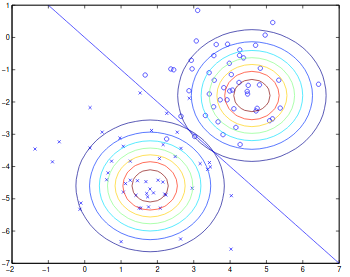
\includegraphics[width=\textwidth]{images/gda}
\end{figure}

\subsection{Discussion: GDA and logistic regression}

The GDA model has an interesting relationship to logistic regression, in fact if we view the quantity 
\[ p(y = 1 | x; \phi, \mu_0, \mu_1, \Sigma) \]
as a function of $x$, we’ll find that it can be expressed in the form
\[ p(y = 1 | x; \phi, \Sigma, \mu_0, \mu_1) = \frac{1}{1 + exp(-\transpose{\theta}x)} \]
where $\theta$ is some appropriate function of $\phi, \Sigma, \mu_0, \mu_1$.

This is exactly the form that logistic regression, a discriminative algorithm, used to model 
$p(y = 1 | x)$ and GDA and logistic regression will, in general, give different decision boundaries
when trained on the same dataset.\newline
We just argued that if $p(x | y)$ is multivariate gaussian(with shared $\Sigma$), then $p(y | x)$
necessarily follows a logistic function and the converse, however, is not true, so $p(y | x)$
being a logistic function does not imply $p(x | y)$ is multivariate gaussian.

This shows that GDA makes stronger modeling assumptions about the data than does logistic regression and 
it turns out that when these modeling assumptions are correct, then GDA will find better fits to the data, 
so it is a better model.

Specifically, when $p(x | y)$ is indeed gaussian (with shared $\Sigma$), then GDA is asymptotically efficient
and informally, this means that in the limit of very large training sets, there is no algorithm that
is strictly better than GDA, in terms of how accurately they estimate $p(y |x)$.

In particular, it can be shown that in this setting, GDA will be a better algorithm than logistic regression
and more generally, even for small training set sizes, we would generally expect GDA to better.\newline
In contrast, by making significantly weaker assumptions, logistic regression is also more robust 
and less sensitive to incorrect modeling assumptions and there are many different sets of assumptions that
would lead to $p(y |x)$ taking the form of a logistic function; for example, if $x | y = 0 \sim Poisson(\lambda_0)$,
and $x | y = 1 \sim Poisson(\lambda_1)$, then $p(y | x)$ will be logistic.

Logistic regression will also work well on Poisson data like this, but if we were to use GDA on such data,
and fit Gaussian distributions to such non-Gaussian data, then the results will be less predictable,
and GDA may (or may not) do well.

Specifically, when the data is indeed non-Gaussian, then in the limit of large datasets, logistic regression will
almost always do better than GDA and for this reason, in practice logistic regression is used more often than GDA.

\section{Naive Bayes}
In GDA, the feature vectors $x$ were continuous, real valued vectors and let’s now talk about a 
different learning algorithm in which the $x_j$’s are discrete-valued.

For our motivating example, consider building an email spam filter using machine learning and here,
we wish to classify messages according to whether they are unsolicited commercial(spam) email, or non-spam email.

After learning to do this, we can then have our mail reader automatically filter out the spam messages and
perhaps place them in a separate mail folder: classifying emails is one example of a broader set of problems
called \emph{text classification}.

Let’s say we have a training set (a set of emails labeled as spam or non-spam) and we’ll begin our construction
of our spam filter by specifying the features $x_j$ used to represent an email.

We will represent an email via a feature vector whose length is equal to the number of words in the dictionary and 
specifically, if an email contains the $j$-th word of the dictionary, then we will set $x_j = 1$ otherwise,
we let $x_j = 0$ so for instance, the vector 
\[ x = \begin{bmatrix}
    1 \\
    0 \\
    \vdots \\
    1 \\
    \vdots \\
    0 \\
       \end{bmatrix} \]
is used to represent an email that contains the words "a" and "buy" but not "aardvark", "aardwolf" 
or "zygmurgy.".

The set of words encoded into the feature vector is called the \emph{vocabulary}, so the dimension of
$x$ is equal to the size of the vocabulary and having chosen our feature vector, 
we now want to build a generative model, so we have to model $p(x | y)$.

If we have a vocabulary of $50000$ words, then $x \in \{0, 1\}^{50000}$ and if we were to model $x$
explicitly with a multinomial distribution over the $2^{50000}$ possible outcomes, then we’d end up 
with a $(2^{50000} - 1)$-dimensional parameter vector so this is clearly too many parameters.

To model $p(x |y)$, we will therefore make a very strong assumption, so we will assume that the $x_i$’s
are conditionally independent given $y$ and this assumption is called the Naive Bayes (NB) assumption,
and the resulting algorithm is called the \emph{Naive Bayes classifier}.

We now have 
\begin{align*}
    p(x_1, \dots, x_{50000} | y) & = p(x_1 | y)p(x_2 | y, x_1)p(x_3 | y, x_1, x_2) \dots 
                                     p(x_{50000} | y, x_1, \dots, x_{49999}) \\
                                 & = p(x_1 | y)p(x_2| y)p(x_3 | y)\dots p(x_{50000} | y) \\
                                 & = \prod _{i=1}^n p(x_i | y) 
\end{align*}
The first equality simply follows from the usual properties of probabilities, the second equality used
the NB assumption and we note that even though the Naive Bayes assumption is an extremely strong assumptions,
the resulting algorithm works well on many problems.

Our model is parameterized by $\phi_{j | y = 1} = p(x_j = 1 | y = 1)$, $phi_{j | y = 0} = p(x_j = 1 | y = 0)$,
and $\phi_y = p(y = 1)$ and as usual, given a training set $\{(x^{(i)}, y^{(i)}) \forall i =1, \dots, m \}$,
we can write down the joint likelihood of the data as
\[ L(\phi_y, \phi_{j | y = 0}, \phi_{j | y = 1}) = \prod _{i = 1}^ m p(x^{(i)}, y^{(i)}) \]
Maximizing this with respect to $\phi_y, \phi_{j | y = 0}$ and $\phi_{j | y = 1}$ 
gives the maximum likelihood estimates
\begin{align*}
    \phi_{j | y = 1} & = \frac{\sum _{i=1} ^ m 1\{x_j^{(i)} = 1 \land y^{(i)} = 1\}}{\sum _{i=1}^m 1\{y^{(i)} = 1\}} \\
    \phi_{j | y = 0} & = \frac{\sum _{i=1} ^ m 1\{x_j^{(i)} = 1 \land y^{(i)} = 0\}}{\sum _{i=1}^m 1\{y^{(i)} = 0\}} \\
    \phi_j           &= \frac{\sum _{i=1} ^ m 1\{y^{(i)} = 1\}}{m}
\end{align*}
Having fit all these parameters, to make a prediction on a new example with features $x$,
we then simply calculate 
\begin{align*}
    p(y = 1 | x) & = \frac{p(x | y = 1)p(y = 1)}{p(x)} \\
                 & = \frac{\left(\sum _{j = 1}^n p(x_j | y = 1) \right) p(y = 1)}
                          {\left(\sum _{j = 1}^n p(x_j | y = 1) \right) p(y = 1) +
                           \left(\sum _{j = 1}^n p(x_j | y = 1) \right) p(y = 0)} 
\end{align*}
and pick whichever class has the higher posterior probability.

Lastly, we note that while we have developed the Naive Bayes algorithm mainly for the case of problems
where the features $x_j$ are binary valued, the generalization to where $x_j$ can take values in 
$\{1, 2, \dots, k_j\}$ is straightforward, so we would simply model $p(x_j | y)$ as multinomial rather
than as Bernoulli.

Indeed, even if some original input attribute were continuous valued, it is quite common to discretize it,
that is, turn it into a small set of discrete values, and apply Naive Bayes.

\section{Laplace smoothing}
The Naive Bayes algorithm as we have described it will work fairly well for many problems,
but there is a simple change that makes it work much better, especially for text classification.

Let’s briefly discuss a problem with the algorithm in its current form, and then talk about how we can fix it
so we consider spam/email classification, and let’s suppose that, after completing the ML course,
you decide to submit the work you did to the NIPS conference for publication (NIPS is one of the top 
machine learning conferences, and the deadline for submitting a paper is typically in late June or early July).

Because you end up discussing the conference in your emails, you also start getting messages 
with the word “nips” in it, but this is your first NIPS paper, and until this time, you had not previously
seen any emails containing the word “nips”; in particular “nips” did not ever appear in your training set
of spam/non-spam emails.

Assuming that “nips” was the $35000$-th word in the dictionary, your Naive Bayes spam filter therefore
had picked its maximum likelihood estimates of the parameters $\phi_{35000| y}$ to be
\begin{align*}
    \phi_{35000 | y = 1} & = \frac{\sum _{i=1}^m 1\{x_{35000}^{(i)} = 1 \land y^{(i)} = 1\}}
                                  {\sum _{i=1}^m 1\{y^{(i)} = 1\}} \\
    \phi_{35000 | y = 0} & = \frac{\sum _{i=1}^m 1\{x_{35000}^{(i)} = 1 \land y^{(i)} = 0\}}
                                  {\sum _{i=1}^m 1\{y^{(i)} = 0\}}
\end{align*}
Because it has never seen “nips” before in either spam or non-spam training examples, it thinks 
the probability of seeing it in either type of email is zero and hence, when trying to decide 
if one of these messages containing “nips” is spam, it calculates the class posterior probabilities, 
and obtains $p(y = 1 | x) = \frac{0}{0}$.

This is because each of the terms $\prod _{j=1}^n p(x_j | y)$ includes a term $p(x_{35000} | y) = 0$ 
that is multiplied into it, so our algorithm obtains $0 / 0$, and doesn’t know how to make a prediction.

Stating the problem more broadly, it is statistically a bad idea to estimate the probability of some event
to be zero just because you haven’t seen it before in your finite training set.

To avoid this, we can use \emph{Laplace smoothing}, which uses 
\begin{align*}
    \phi_{j | y = 1} & = \frac{\sum _{i=1}^ m 1\{x_j^{(i)} = 1 \land y^{(i)} = 1\} + 1}
                              {\sum _{i=1}^ m 1\{y^{(i)} = 1\} + 2} \\
    \phi_{j | y = 0} & = \frac{\sum _{i=1} ^ m 1\{x_j^{(i)} = 1 \land y^{(i)} = 0\} + 1}
                              {\sum _{i=1}^m 1\{y^{(i)} = 0\} + 2} \\
\end{align*}
In practice, it usually doesn’t matter much whether we apply Laplace smoothing to $\phi_y$ or not,
since we will typically have a fair fraction each of spam and non-spam messages, so $\phi_y$ 
will be a reasonable estimate of $p(y = 1)$ and will be quite far from 0 anyway. 
%If we are given a training set{(x(i), y(i));i= 1, . . . , m}wherex(i)=(x(i)1, x(i)2, . . . , x(i)ni) (here,niis the number of words in thei-training example),the likelihood of the data is given byL(φy, φk|y=0, φk|y=1)  =m∏i=1p(x(i), y(i))=m∏i=1(ni∏j=1p(x(i)j|y;φk|y=0, φk|y=1))p(y(i);φy).Maximizing this yields the maximum likelihood estimates ofthe parameters:φk|y=1=∑mi=1∑nij=11{x(i)j=k∧y(i)= 1}∑mi=11{y(i)= 1}niφk|y=0=∑mi=1∑nij=11{x(i)j=k∧y(i)= 0}∑mi=11{y(i)= 0}niφy=∑mi=11{y(i)= 1}m.If we were to apply Laplace smoothing (which needed in practice for goodperformance) when estimatingφk|y=0andφk|y=1, we add 1 to the numeratorsand|V|to the denominators, and obtain:φk|y=1=∑mi=1∑nij=11{x(i)j=k∧y(i)= 1}+ 1∑mi=11{y(i)= 1}ni+|V|φk|y=0=∑mi=1∑nij=11{x(i)j=k∧y(i)= 0}+ 1∑mi=11{y(i)= 0}ni+|V|.While not necessarily the very best classification algorithm, the Naive Bayesclassifier often works surprisingly well. It is often also a very good “first thingto try,” given its simplicity and ease of implementation.


% Chapter 5 Generative Algorithms
%    \input{supportVectorMachine}% Chapter 6 Support Vector Machine
%    \chapter{Neural Network}
Neural Network is used to study and model biological systems and learning processes (used in Philosophy, Psychology and neurobiology, cognitive science, Computational neuroscience).
We use Neural Network to introduce effective ML systems/algorithms, often losing a strict biological realism, and that is concern on Statistics, Artificial Intelligence, Physics, Math., Engineering, and where ML, computational  and algorithmic properties are essential.

We will analyze in this course \emph{ANN (Artificial Neural Networks)} is indeed a (flexible) Machine Learning tool (in the sense of approximation of functions:
it realizes a mathematical functions h(x) with special properties), infact NN can learn from examples, are a universal approximators (Theorem of Cybenko: flexible approaches for arbitrary functions),
can deal with noise and incomplete data (Performance degrade gracefully under adverse operating conditions), and in the end NN can handle  continuous real and 
discrete data for both regression and classification tasks.\newline
NN is a successful model in ML due to the flexibility in applications and encompasses a wide set of models, so it is a paradigm (in the class of subsymbolic approaches).

Each node in NN is called neuron or unit (see figure \ref{img:neuron}) and the input are from extern source or other units (IR) and the connection is done by weight w
(free parameters, that can be modified by learning (synaptic strength)), where we have that the weighted sum $net_i$ is called the net input to unit $i$,defined as 
\[ net_i(x) = \sum _j w_{ij} x_j \]
and note that $w_{ij}$ refers to the weight of the unit $i$ and the function $f$ is the unit's activation function(e.g linear, LTU, ...), where the result
of $f(net_i)$ is the output $o_i$ of a node $i$.

\begin{figure}
    \caption{Structure of ANN node}
    \label{img:neuron}
    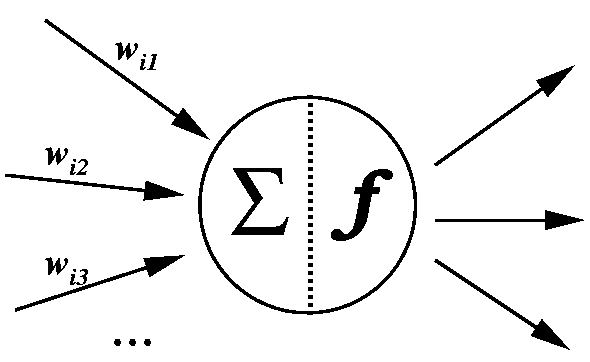
\includegraphics[width=\textwidth]{images/artificialNeuron}
\end{figure}
Every Boolean function can be represented by some network of interconnected perceptrons, only two levels deep is sufficient (or more can be more efficient*), but single layer 
cannot model all the possible functions, like for example XOR function, so we need hidden layers in NN to represent complex tasks.

There are two kinds of method for learning:
\begin{description}
    \item[Adaline (Adaptive Linear Neuron invented by Widrow, Hoff):] linear, LMS direct solution and gradient descent solution, as we have introduced in Regression and Classification chapter,
	    							      that is not proved to converge but only with an approximation.
    \item [Perceptron(Rosenblatt):] non-linear (with hard limiter or Threshold activation function) and can be used only for classification and it is ensured that converge.
	    			    Perceptron represent linear decision boundaries, can solve only linearly separable problems and it has as activation function the following
				    \[ f = sign(\transpose{\theta}x) \]
				    with values that can be $1$ (positive class) or $-1$ (negative class).
					
				   Perceptron learning algorithm consist to compute the predicted output $out = sign(\transpose{\theta}x)$ and if $out \neq y$ we update the weights $\theta$ using
				   \[ \theta = \theta + \frac{1}{2} \eta (y - sign(\transpose{\theta}x)) x \]

				   \begin{thm}
					   Perceptron is guaranteed to converge (classifying correctly all the input patterns) in a finite number of steps if the problem is linearly separable.
				   \end{thm}
\end{description}
Common activation function are the linear, logistic, $\tanh$ function but it is also used the softmax function, RELU(Rectified Linear Unit) and gaussian function,
anyway usually we will use a different activation between output and hidden units and common choice are $\tanh$ for hidden unit and linear for output unit.

We will analyze standard feedforward NN, where the architecture of a NN defines the topology of the connections among the units and the two-layer feedforward neural network 
described in \ref{img:feedforward} and \ref{img:feedEquation}, corresponds to the well-know MLP(Multilayer Perceptron) architecture: the units are connected by weighted links 
and they are organized in the form of layers. 

The Hypothesis space of feedforward NN is the continuous space of all the functions that can be represented by assigning the weight values of the given architecture and many early results
(Cybernko 1989 and so on) estabilish that a single hidden-layer network (with logistic activation functions) can approximate (arbitrarily well) every continuous (on hyper cubes) function
(provided enough units in the hidden layer) so a MLP network can approximate (arbitrarily well) every input-output mapping (provided enough units in the hidden layers).

The univ.approx. theorem is a fundamental contribution•It show that 1 hidden layer is sufficient in general, but it does notassure that a “small number” of units could be sufficient (it does not provide a limit on such number)•It is possible to find boundaries on such number (for many f. families)•But also to find “no flattening” results (on efficiency, not expressivity):–cases for which the implementation by a single hidden layer would require an exponential number of units (w.r.t n input dim.), or non-zero weights,–while more layers can help (it can help for the number of units/weights and/or for learning such approximation)–But is it easy to optimize (training) a MLP with many layers

NN with backprogationlearning algorithm: •Generally related to the smoothnessproperties of functions:–Small input variations small output variations–E.g. a locally limited value of the first derivative.–A very common assumption in ML•Why make sense? A target function that is not Non-smooth: random number generator generalization cannot be achieved

The learning algorithm allows adapting the free-parameters wof themodel, i.e. the values of the connection-weight, in order to obtain the best approximationof the target function. •In the ML framework this is often realized in terms of minimizationof an error (or loss) function on the training data set.•The problem is the same we have seen for the other models (repetita), starting again with the simple LMS case:–Givena set of ltraining example  (xp,dp)  and a loss function (measure) L –Find: The weight vector wthat minimizes the expected loss on the training data:

Note that in general:•Loading problem: (“loading” a given set of tr data into the free par. of the NN) –given a network and a set of examples –answer yes/no: is there a set of weights so that the network will be consistent with the examples?•The loading problem is NP-complete (Judd, 1990)•This implies that hard problems cannot be “solved” ! •In practice networks can be trained in a reasonable amount of time (see the back prop alg.) although optimal solution is not guaranteed

Find  w by computing the gradient of the error (loss) function•Epoch: an entire cycle of training pattern presentation•Nice properties (also for programming):–easy because of the compositional form of the model–keep track only of quantities local to each unit (by local variables) modularityof the units is preserved

To train an multilayer feedforward NN it has been introduced in \cite{backpropagation} the \emph{Backpropagation} algorithm, that it is an evolution
BACKPROPAGATION

General problems:•The model is often over-parametrized•Optimization problem is not convex and potentially unstable

Hyper-parameters= values that youhave to set-up to run the training

Starting values (winitialin the basic alg.)•(!)Initialize weights by random values near zero –Avoid for W: all zero, high values, or all equals (symmetry): these can hamper the training•E.g. in the range [-0.7,+0.7] (for standardized data, see later)•Considering the Fan-in : e.g. range * 2/fan-in–Not if fan-in is too large–Not for output units (else delta start close to zero !)•Other heuristics ...orthogonal matrix, .... (enjoy if  you like) –Very popular among practitioners: Glorot, BengioAISTATS 2010: 0 for biases and w random from Uniform distribution in [-1/a, +1/a] with a=sqrt(fan-in) or (later results) a depending also on fan-out ... •Note (practicalfor the first part of the project): a very small NN (very few units) can have a stronger dependencies w.r.t.initialization

Multiple Minima•Loss is not convex: many local minima•The result depends on starting weight values•Not really a big issue –you can see the final training error–a “good” local minima is often sufficient (see the next slide)•(!)Try a number of random starting configurations(e.g. 5-10 or more training runs or trials)•Take the mean results (mean of errors) and look to varianceto evaluateyour model and then, if you like to have only 1 response :–you can choose the solution giving lowest (penalized) error (or the median)–You can take advantage of different end points by an average (committee) response: mean of the outputs/voting

ndeed in ML we don’t need neither local or global minima on Rempas we are searching the min of R(that we cannot compute). –Often we stop in a point that has not null gradient and hence also  neither a local or global minima for the empirical (training) error.•The NN build a variable size hpspace (see at the end of NN-first part slides)→it increases VC-dim during training →the training  error decreases toward zero not because we reach a global minimum but because the NN becomes too complex (high VC-dim)•Stopping before this condition of overtraining(and hence overfitting) is needed

For Batch version: sum up all the gradients of each pattern over an epoch and then update the weights (Dwafter each “epoch” of lpatterns)•Stochastic/on-lineversion: upgrade wfor each pattern p (by Dpw)  without wait the total sum over l:–It makes progress with each examples it looks at: it can be faster, but it need smaller eta

Batch version: more accurate estimation of gradient •On-line or Stochastic version:  since the gradient for a single data point can be considered a noisy approximation to the overall gradient, this is also called stochastic(noisy) gradient descent. Zig-zag (stochastic) descent (see figures in the next slide)–It can help avoiding local minima–A different order of patterns in different epochs should be used  (to avoid a bias/drift in the gradient descending)–(!)Usually random order (shuffling the patterns)•Many variationsexist: for instance –Stochastic Gradient Descent (SGD) using minibatch –mb (few training examples) for each step of gradient descent

Minibatchstochastic method →akaSGD–Use random sampling to implement the minibatch(unbiased estimation). By shuffling  (at the beginning for all the TR data or for each mini batch)–With very large TR set or online streaming →even no epochs!–Along with the advantage of gradient descent (linear cost wrtexamples) SGD with mbis a key factor in extending learning to very large data sets (over millions of examples) because mb(and hence the cost of each SGD update) does not depend on l : typically just mini-batch  and  (again) no epochs repetition

Batch: more accurate estimation of gradient →higher eta value•On-line:it can make the training faster but can be more unstable →smaller eta valueMore in general (on the eta values):•High versuslow etavalues :  fast (but possible unstable if too large) versusstable (but possible too slow if too small)•And we will see various techniques to improve the convergence speed•Anyway, still you ask for some values ?!?Typically, search in the range [0.01-0.5] in LMS

Learning curve, plotting errors during training, it allows you to check the behavior in the early phases of the model design for your task at hand (preliminary trials)–Please check the Learning Curve whiletraining a NN! •We are now looking to the curve quality and convergence speed: of course the absolute value for the training error depends also on the model capacity (see later for the number of units, regularization etc.) and the other hyperparameters

Practical approach: it is useful to use of the mean(average) of the gradients over the epoch: it helps to have an “uniform” approach with respect to the number of input data
Repetitafrom “Gradient descent algorithm”: dividing by l  correspond to have the LeastMeanSquares–Note that it is equivalent to  have: eta/l–Off course divide by mb for mini batch•Note that if you compare on-line with batch using LMS (i.e. /l), then using on-line training will require much smaller eta to be comparable!!!! (in order of the same factor /l used to divide the gradient in the batch version

Momentum –NesterovMomentum2.Variable learning rate (initially high then decrease)3.Adaptive learning rates (change during training and for each w) (see also in Deep Learning  lectures)4.In NN with many layers (see deep learning lectures): –It can be varied depending on the layer (higher for deep layers) or fan-in (higher for few input connections)

Faster in plateaus: same sign of grad. for consecutive iterations →momentum increase the delta •Damps oscillations: stabilizing effect in directions that oscillate in sign•Inertia effect: Allow us to use higher eta (learning parameter: e.g. 0.2-0.9)
Alfa: 0<momentum parameter <1 e.g 0.5 -0.9

Effect on a canyon of the error surface (#poor conditioning of the Hessian matrix).•In redthe path with the momentum, lengthwise traversing the valley toward the minimum•Instead of zig-zag along the canyon walls (following the blackdirections given by the gradient)

Momentum born with “batch” learning, and it is commonly assumed that helps more in  batch mode •In the on-lineversion can be used but it is connected to a moving average of the past gradients concept to smooth out the stochastic gradient samples [e.g. see it in the form grad= alfa grad+(1-alfa) gradnow]•It smooths the gradient over different examples (a different meaning w.r.t.the batch version that uses the same batch of examples)•You can use it multiplying by eta (as usual) to obtain the  DeltaW

For Minibatch: moving average of past gradients over the progressive minibatchs(that have different examples, not the step before for the same examples as for batch)

Using mini-batch →the gradient does not decrease to zero close to a minimum (as the exact gradient can do)•Hence fixed learning rate should be avoided:•For instance, we can  decay linearly eta for each step until iteration tau (), using =(step s)/:•Then stop and use fix (small) •Set-up: as ~1% of 0, few hundred steps•And 0 ? Again: no instability/ no stuck trade-off (preliminary trials or grid-search

Adaptive Learning Rates•Automatically adapt the learning rate during training•Possibly avoiding/reducing the fine tuning phase via hyperparameters selection•Use separate etafor each parameter

As any iterative approaches.... Basic SGD is generally efficient (linear in the number of free parameters)  but depends on the number of training data and on the number of epochs

Use the second order derivatives (Hessian matrix): more information about the curvature of the objective function →better descent (Newton's methods )–But the Hessian can be too large (i.e. computationally expensive), and see the next “saddle points” slideIn the form of approximatesecond order methods we find:•Approx. Newton's methods (also Gauss-Newtonand Levenberg-Marquardt  approximation)•Hessian free approaches (without computing H and H-1)–Conjugate gradients•can be nice for faster converge! (see e.g. in “Numerical Recipes in C”).–Quasi-Newton methods: BFGS (Broyden–Fletcher–Goldfarb–ShannoAlgorithm

Dip. InformaticaUniversity of PisaSaddle points #techMore intriguing discussion on saddle points (see e.g. 8.2 Deep Learning book) i.e. Gradient (close to) zero but not a local minima•Saddle points can grow exponentially (wrtto local minima) in high dimensional spaces •Newton search for (jump to) gradient zero points –more sensible to find saddle points•This can explain why (standard) second-order methods (looking to Hessian, e.g. Newton’s method) have not succeedin replacing gradient descent for NN training •Instead, Gradient descent empirically shows to escape saddle points [...]•But the length of the training path can be high for many other reason not related to local minima or saddle points (small gradient values), such as time to “circumnavigate” local maxima and so on.

For optimization: Don’t worry, the main basics approaches e.g. with (!), often are enough if you apply them correctly–The experience with well-know techniques have a major role than sophisticated approaches that you cannot manage. –The optimization technique is relevant only if there are obstacles for training. Validation will have a major role than the optimization on the training set (we will have next lectures on this): remember, optimize on the training data is not our purpose!–The others are an opportunity to explore different approaches (especially using libraries) •SGD with momentum (ad we will see regularization) is in any case a starting point, also as comparison if you move toward other approaches

The basic is the used loss (loss<k): the best if you know thetolerance of data (expert knowledge)•Other e.g.–Max (instead of mean) tolerance on data–Classification: Number of misclassified (error rate)–No more relevant weight changes/ near zero gradient (Euclidian norm of gradient < epsilon)/ No more significant error decreasing for aepoch (e.g. less than 0.1%):NOTE: may be premature (e.g. if eta is too small)!It can be applied observing k epochs.•(!)In any case stop after an excessive number of epochs •Not necessarily stop with very low training error

The control of complexity  is our main aim to achieve the best generalization capability•For instance  we need to add some regularization: •this isachieved directly through a penalty term, or indirectly by early stopping.•+ model selection(cross-validation) on empirical data to find the trade-off

Start learning with small weights (symmetrybreaking) •The mapping input→outputisnearlylinear: –numberof effectivefree parameters(and VC-dim) nearlyasin perceptron•Asoptimizationproceedshiddenunitstendto saturate, increasingthe effectivenumberof free parameters(and introduce non-linearities) and henceincreaseVC-dim•A variable-size hypothesisspace

Early stopping: use a validation setfor determining when to stop (at the validation error increasing: ... quite vague!)–Use more than one epoch before estimating (patience)–Backtracking approaches–Note that since effectivenumb. of parameters  grows during the course oftraining, halting training correspond to limit the effective complexity–See “Early Stopping—ButWhen?» L. Prechelt,  LNCS 2012–We will discuss also later about Early Stopping2.Regularization (on the loss : our main warhorse!)3.Pruning methods: see later

Training →weight increases: We can  optimize the loss considering the weight values•A well know principled approach (related to Tikhonov theory, again):•Add a penalty term to the error function:•Effect: weight decay (basically add 2wto the gradient for each weight)•Chose the lambda regularization  parameter (generally very low value, e.g. 0.01):  selected by the model selection phase (cross-validation)•Note: if applied to linear model →it is the ridge regression (see lect.on linear models)•More sophisticated penalty terms have been developed

Note that often the biasw0is omitted from the regularizer(because its inclusion  causes the results to be not independent fromtarget shift/scaling) or it may be included but with its own regularizationcoefficient (see Bishop book, Hastie et al. book)•Typically apply it  in the batch version •For on-line/mini-batchtake care of possible effects over many steps (patterns/examples): hence to compare w.r.t. batch version in a fair way do not force equal lambda but it would be better to uselambdax (mb/#total patterns l )–Of course if you choose lambda by model selectionthey will  automatically select different lambda for on-line and batch (or any mini-batch)

Does the regularization help the convergence stability?It is important  to highlight that the regularization is not a technique to control the stabilityof the training converge but, as you well know, it allows the control of the complexityof the model  (measured by the VC dimension according to the SLT theory), which is related to the number of weights and values of the weights in NNs.2.Better Early Stopping (E.S.) or Regularization (R.)?We will discuss later, butnote that the E.S. needs a VL set  to decide the stopping point, which sacrifices a part of data. The R. in the Loss is a principled approach: it allows the VL curve to follows the TR curve (provided that you avoid that the VL curve is close to TR curve due to  underfitting with a too high lambda) so that you don’t need of the E.S. heuristic and you can stop at training convergence

Number of Units•Related to the control of complexityissue !!!•Related also to the input dimension and to the size of the TR data set In general: a “model selection”issue•The number of units along with regularization parameter can be selected by a cross-validation, i.e. the model selection phase (on a validation set)–To few hidden units →underfitting; to many →overfitting (can occur)–The number of units can be high if appropriate regularization is used•Constructive approaches: the learning algorithm decides the number starting with small network and then adding new units•Pruning methods: start with large networks and progressively eliminate weights or units

Constructive approaches•Incrementalapproach: algorithms that build a network starting with a minimal configuration and•add new units and connections during training

An exemplificative and effective approach :•the Cascade Correlationlearning algorithm•Start with a minimum networks•Add units if they are needed until the error is low.•The CC alg. learns both the network weights and network topology (number of units)–automatic determination of network dimension and topology: CC allows to deal with hypothesis spaces of flexible size, since the number of hidden units is decided by the learning algorithm;–training of a single unit for each step

The CC algorithm•Start withN0 network, a network without hidden units: Training of N0. Compute error for N0. If N0 cannot solve the problemgo to N1.•In the N1 networka hidden unit is added such that the correlationbetween the output of the unit and the residual error of networkN0 is maximized (by training its weights, see next slide). •After training, the weights of the new unitare frozen(they cannot be retrainedin the next steps) and the remaining weights (output layer) are retrained.•If the obtainednetwork N1cannot solve the problem, new hidden units are progressively addedwhich are connected withall the inputs and previously installed hidden units. •The processcontinues until the residual errors of the output layer satisfy a specified stoppingcriteria(e.gthe errors are below a given threshold).The method dynamicallybuilds up a neural network and terminates once a sufficientnumber of hidden units has been found to solve the given problem.Cascade of units

 the algorithm works interleavingthe minimization of the total error function (LMS), e.g. by a simple backpropagation training of the output layer, and the maximization of the (non-normalized) correlation, i.e. the covariance, of the new inserted hidden (candidate) unit with the residual error

 The role of hidden units is to reduce the residual output error –It solves a specific sub-problem–It becomes a permanent “feature-detector”•POOL: Typically, since the maximization of the correlation is obtained usinga gradient ascent technique on a surface with several maxima, a pool of hidden units istrained and the best one selected. This help avoid local maxima. •Greedy algorithms: easy to obtain converge, may also find a minimal  number of units but it may lead into overfitting (need regularization)

 Dip. InformaticaUniversity of PisaA. MicheliInput/Output•Preprocessing  can have large effect•For different scale values, normalization via : –Standardizations (often useful):For each feature we obtain zero mean and standard deviation 1: v-mean /standard dev.–Rescaling: [0,1] range: v-min /(max-min)

 Regression: Output linearunit(s)–(1 unit or more output units for multiple quantitative response)•Classification: 1unit  (binary) or 1-of-K with multioutput –Sigmoid →choose the threshold to assign the class–Rejection zone (is possible, se slide on sigmoidal functions)–1-of-K encoding: to choose the winner class take the highest value among the output values–Often symmetric logistic (TanH) learn faster (see Haykinbook)–0.9 can be used instead of  1 (as d value) to avoid asymptotical convergence      (-0.9 for –1 for TanH, or 0.1 for 0 for logistic)Of course, target range must be in the output range of units

Black-box problem (inherent inability/difficulty to explain, i.e. it is difficult to interpret the acquired knowledge):–extraction and representation of knowledge for human experts–related to the current trend in the research for interpretability of ML models and the “explainable artificial intelligence” issue

Architectural design :–Constructive/pruning methods to optimize the architecture–New approaches (SVM)•Training process dependency: training realization have effect on the final solution

 Not the best for Missing data: standard strategies including removing data, imputations, ...•When to consider NN: –Input is high-dimensional discrete or real-valued / classification and regression tasks–Possibly noisy data–Training time is unimportant–Form of target function is unknown–Human readability of result is unimportant–The computation of the output based on the input has tobe fast



% Chapter 7 Neural Network
\end{document}
